\chapter{AcCAPPCHA}
AcCAPPCHA is a verification that works like a key-logger. This type of programs is usually malicious and intended to be used by an attacker to acquire information about the user's activity. This application analyses the sequence of keys inserted by exploiting side-channel information. Its implementation depends on the party, that the hacker wants to attack\cite{keylogging}, and that could be:
\begin{itemize}
\descItem{The user}
{these attacks are based on the exploitation of physical information related to the typing state. For example, they can use electroencephalography (EEG), motion of the wrist in the smartwatches, video with keyboard line-of-sight and WiFi signal distortion.}
\descItem{The keyboard}
{these attacks are based on analysis of signals coming from the keyboard. For example, acoustic emanations can be exploited by using external physical sensors.}
\descItem{The host}
{these attacks are based on the physical access of the attacker to the victim machine. For example, the process footprint, the CPU load and other micro-architectural analysis can be exploited in this attacks.}
\descItem{The network}
{these attacks exploit the packets exchanged in the client-server communication. For example, a network packet can be related to a keystroke revealing the key press time of the victim and the payload size of the server response.}
\end{itemize}
Analysing the previous key-logger based on side-channel information, attacks mentioned in Section \ref{chapter:SideCH} and the structure of Invisible CAPPCHA in Section \ref{chapter:InvisibleCAPPCHA}, I design this new implementation of CAPTCHA. It exploits acoustic side-channel of microphone to implement a particular type of keylogger that ensures that Authentication phase would be performed by a human user.\\
The whole implementation was created using \texttt{Python} language. The structure and the behaviour of AcCAPPCHA are similar to the ones proposed in Invisible CAPPCHA because they are both based on the evaluation of signal, detected by some sensor (motion sensors for Invisible CAPPCHA and microphone for AcCAPPCHA). With respect to Invisible CAPPCHA the program can perform also a classification of the audio signal using neural networks. The two phases of the verification are:
\begin{itemize}
\item{Evaluation of the user's activity}
\item{Communication with the remote service}
\end{itemize}
In the second phase, the username and the password of the user will be signed through ECDSA and sent by client to the authentication service if and only if the insertion was performed by a human.

\section{Evaluation of the user's activity}
The CAPPCHA records two audio signals: the first one created during the insertion of the password by the user and the second one created before this activity for noise evaluation. The second signal is exploited to evaluate a noise threshold useful for the computation of amplitude peaks in the first audio.
During the insertion of the password, the instants of the time when each character was typed by the user are stored. 

\subsection{Time correspondence}\label{design:time_correspondence}
Before asking the user to insert the password, the program records an audio file of 1 second, called \texttt{noise signal}, from the built-in microphone of the laptop. The remaining verification procedure is performed by two threads simultaneously, during password insertion. The first one is continuously waiting for the insertion of a character of the password by the user until he types CARRIAGE RETURN\textit{'\r'}).\\
Immediately after a key is pressed, the time instant of this action, related to the Epoch of the PC, is stored to be used later. The sequence of time instants stored by the thread is named $x=(x_0, ..., x_{|password|-1})$. The second thread records an audio signal, called \texttt{user activity}, using the same hardware previously mentioned. This task begins its activity before the request of the password to the user and ends after the moment in which the first thread detects a CARRIAGE RETURN.\\
From now on, the application has all it needs to understand if the user is a human or not. In fact the verification is performed by looking if there exists a sequence of time instants of the peaks in the signal recorded in parallel to the insertion of the password and the time instants manually stored for each character.\\
In particular \texttt{noise signal} will be analysed by finding its maximum value, called $thresh_N$, and then \texttt{user activity} will be analysed by considering only the samples with values higher than $thresh_N$. These sample will be grouped in several disjoint windows of maximum width equal to 5 ms. For each group \textit{i}, the application finds the sample with the highest value, $peak_i$. For example, given \textit{the sampling period or interval} $t_s$ and a specific group of samples: $$x_i = (x_t, x_{t+t_s}, ..., x_{t+\lceil \frac{5ms}{t_s}\rceil * t_s})$$
the application computes $t_i= argmax(x_i)$.\\
Given the sequence of computed time instants relative to peaks of each group $t=(t_0, t_1, ..., t_{n-1})$, $n$ number of windows and $|password|$ the size of the password, there is a \textbf{time correspondence} if if there exists a subset of it $t^{*}=({t*}_0, ..., {t*}_{|password|-1})$ that matches with the sequence of time instants stored during the password insertion. The algorithm used to find a time correspondence is reported next:
\begin{algorithm}[h]
\DontPrintSemicolon\footnotesize
\KwIn {$\mathtt{x =(x_0, x_1,..., x_{|password|-1})=}$ time instants stored by first thread\newline
$\mathtt{t =(t_0,t_1,...,t_{n-1})=}$ time instants relative to peaks of each group\newline
$\mathtt{threshold=}$ threshold with respect to stored time instant\newline}
\KwOut {$\mathtt{true}$ if human, $\mathtt{false}$ otherwise\newline}
\BlankLine
$\mathtt{y =(y_0, y_1,..., y_{|password|-1})}$ where $y_i=x_i-x_0$\;
\BlankLine
\If{$n<|password|$}{
\textcolor{blue}{\emph{\\Number of found peaks lower than number of characters of the password}}\;
    \BlankLine
    \Return $false$\;
    \BlankLine
}
\BlankLine
\textcolor{blue}{\emph{//Search of subsequence}}\;
\For{$i\leftarrow 0$ \KwTo $n-1$}{
\BlankLine
 \If{$(n-i)<|password|$}{
 \textcolor{green}{\emph{//Not enough peaks from $t_i$ on to be analysed to find the time correspondence}}\;
    \BlankLine
    \Return $false$\;
    \BlankLine
 }
 \BlankLine
 \textcolor{red}{\emph{//$t_i$ already verified}}\;
 $\mathtt{j\gets} i+1$\;
 $\mathtt{count\gets} 1$\;
 \BlankLine
 \While{$count < |password| \wedge j < n$}{
  \BlankLine
  \If{$(n-j)<(|password|-count)$}{
   	\textcolor{orange}{\emph{//Not enough peaks from $t_i$ on to be analysed to find the time correspondence}}\;
   \BlankLine
   $\mathtt{break}$  
   \BlankLine
  }
  \uIf{$\mathtt{(t_j-t_i)}<(y_{count}-threshold)$}{
   	\textcolor{brown}{\emph{//Too less time between the time instant of the first character and the time instant of the \textbf{count}-th character}}\;
    \BlankLine    
    $\mathtt{j}\gets j+1$\;
    \BlankLine
  }
  \uElseIf{$\mathtt{(t_j-t_i)}<(y_{count}+threshold)$}{
	\textcolor{brown}{\emph{//Time correspondence}}\;
    \BlankLine
    $\mathtt{count}\gets count+1$\;
    $\mathtt{j}\gets j+1$\;
    \BlankLine
  }
  \Else{
    \textcolor{brown}{\emph{//Too much time between the time instant of the first character and the time instant of the \textbf{count}-th character.}}\;
    \BlankLine
    $\mathtt{break}$
    \BlankLine
  }
  \BlankLine
  \If{$\mathtt{count =} |password|$}{
    \textcolor{purple}{\emph{//Time correspondence found}}\;
   \BlankLine
   \Return $true$\;
   \BlankLine
  }
  \BlankLine
 }
}
 \caption{Time correspondence}\label{AcCAPPCHA:time_correspondence}
\end{algorithm}
\clearpage
\subsection{Deep learning}
In the following sections, there is a detailed explanation of the main phases followed by the application:
\begin{itemize}
\item{Data acquisition}
\item{Extraction of features}
\item{Neural network}
\item{Verification}
\end{itemize}

\subsubsection{Data acquisition}
To create a program that record audio while user type something, I created \texttt{DatasetAcquisition.py} source file containing the relative class. After instantiating an object of the class \texttt{AcquireAudio}, it applies \texttt{record} method to this instance.\\
Inside this method, two different program are run in parallel: the first one is a key-logger that is used to classify all the recorded audio files in some directories and the second one that records an audio file during keys typing. The update of private members of the class is guaranteed through the use of the mutual exclusion (mutex) management. The keylogger in the first task requires the access to the operating system signals generated by typing a key on the keyboard. It has the only purpose to continue the acquisition of the audio files even if a special key is pressed (for example F3 button).\\
The choice of running two different tasks in parallel was given by the need of recording audio before the start and after the end of password insertion by the user. Each recorded audio can contain several audio peaks related to multiple insertion of the same key but, during the acquisition of training and test set, I record one audio file for each key pressed.\\
Hence in this particular case, the key-logger waits for the insertion of a single key by the user and then reports it to the thread that performs audio recording. This last task also closes the audio stream and stores the audio signal into a \textit{wav} file named with a progressive number. All the audio files are dynamically organized into a set of subfolders of the output directory, each one with the name of the respective typed key.\\
The recording phase was performed using directly the built-in Realtek microphone and the keyboard of my MSI GL63 8RD laptop. The names of the subfolders/labels, in which each audio file of a pressed key is inserted, are reported in Appendix \ref{chapter:keymapping}.\\
Looking at Table , we can see that the keylogger changes its behaviour mapping each key to an ASCII string of upper or lower alphabetic characters because otherwise many keys would be mapped into invalid names of folders (for example, the key \textit{'.'} is now mapped into the label \textit{'POINT'}). In the table, there are two columns of labels: the first one related to the label seen by the key-logger, the second one related to the label assigned by me to each key. The reason why these labels differ for some entry are:
\begin{itemize}
\descItem{higher accuracy for spatial distribution of the keys on the keyboard}{for example, \textit{'INSERT'} and \textbf{'0\_INSERT'} (with Num lock on) would be mapped into \textit{'INSERT'} by the key-logger but they are considered different thanks to the final mapping;}
\descItem{improve the classification of keys made by key-logger}{for example, \textit{'ALT'} label is wrongly mapped into \textit{'SHIFT'} by key-logger.}
\descItem{solve the problem of keys mapped only by hardware}{\textit{FN} is the only key with this problem. The key-logger doesn't detect any pressed key, when \textit{FN} is inserted. Hence, I needed to typed it and then another key to be sure that recording for \textit{FN} was performed. Then I made another python script to resize the audio signal and remove the useless second peak.}
\end{itemize}
The last two reasons are very important because they highlight also the power of acoustic side-channel. If an attacker implements an high-level key-logger exploiting also microphone information, the accuracy of its software can increase very much.\\
In fact the hacker could collect a dataset of recordings of pressed keys on the same type of the victim's keyboard and then could train a Neural Network, that will be add in its malicious code. For each key, I record 200 audio signals obtaining a dataset of 20400 audio files. To improve the accuracy of the prediction for the neural network, I performed also Data Augmentation of the audio signals used for the training phase. I tried two approaches: 
\begin{itemize}
\descItem{Time-shift}{from each audio signal I created 4 new audio signals obtained by applying a time-shift respectively of 0.5, 1.0, 1.5 and 2.0 seconds.}
\descItem{Introduction of Gaussian noise}{from each audio signal I added a sequence of random samples from a Gaussian distribution, with standard deviation equal to 150 and mean 0, generating four new audio signals.\\
}
\end{itemize}
Using these approaches I have a training set of 2000 audio signals for key, composed respectively by the following datasets:
\begin{itemize}
\item{200 audio signals manually recorded by me}
\item{800 audio signals obtained by time-shift technique}
\item{800 audio signals from introduction of Gaussian noise}
\end{itemize}
The accuracy of the Neural Network trained on audio signals of both first and second datasets is higher than the one related to the Network trained on first dataset only.  The efficiency of the Neural Network trained on first and third dataset is worst than the one related to the network trained on first dataset only because the third dataset introduces many sequences of FFT coefficients that are very similar even if they are related to different keys. Hence I used only the network trained on the first dataset and both on the first at the second dataset as prediction model. So having 102 keys, I had respectively a dataset of 20400 and 102000 audio files.

\subsubsection{Classification}
When pressed each key of the keyboard produces a variation of the signal, called \textit{press peak}, for a time window of about 8-10 ms\cite{keyboard_acoustic}. This signal trend can also be divided in three consecutive and distinctive areas:
\begin{itemize}
\descItem{touch peak}{peak in a window of 2-3 ms, caused by the finger touching the key}
\item{\textbf{noisy meaningless area}}
\descItem{hit peak}{peak in a window of 2-3 ms, caused by the finger and the key hitting the keyboard supporting plate.}
\end{itemize}
To obtain a prediction of each key pressed by the user, we can extract information from the touch peak, that is the most significant, and the hit peak, that increases the information related to the pression.\\
Following the idea of Asonov and Agrawal, I exploit deep learning to classify each pressed key. I use three different approaches, the first two were taken from the work of Asonov and Agrawal and the last one was based on modern sound classification techniques.\\
Respectively to the method used, the feature for each key was composed by:
\begin{itemize}
\item{FFT coefficients of the touch peak}
\item{FFT coefficients of the hit peak and the touch peak}
\item{Features obtained from the hit peak and the touch peak using a deep learning pre-trained model}
\end{itemize}
In the first two cases, the coefficients are extracted from a window of 3 ms around the peaks and then they are normalized in floating point values in range $[0, 1]$ (see Figure \ref{AcCAPPCHA:feature_example}).\\
In the third case, the touch peak and the hit peak samples were concatenated, creating a new signal on which the spectrogram is computed. From the spectrogram, I extract a feature composed by 512 values through the use of VGG16 pre-trained convolutional neural network.\\
In this way, I remove the last fully connected layers, used for classification of other task, and take the intermediate results as feature. The reason of this approach is that a pre-trained network already extracts very well features for classification of a lot of common immages and so it can extract features better than a NN created from scratch.
\begin{figure}[h]
     \centering
     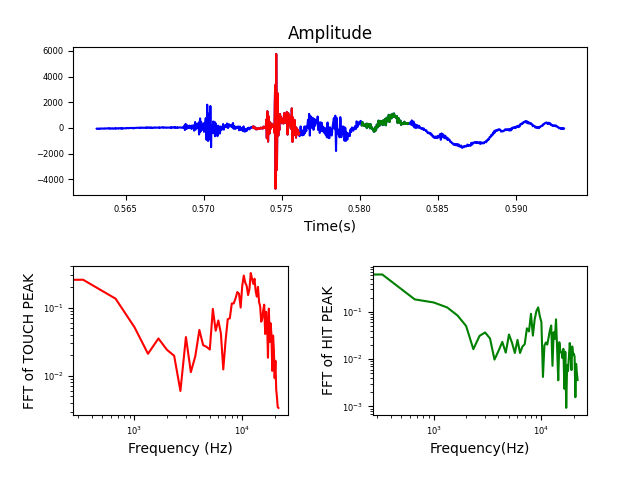
\includegraphics[width=.9\linewidth]{Images/Design/feature_example}
     \caption{\footnotesize{Example of normalized FFT computation for the touch and the hit peak.}}\label{AcCAPPCHA:feature_example}
\end{figure}

\subsubsection{Verification}
The audio signal taken, during the insertion of the password, is analysed and then organized in windows as specified in the previous Section, but the prediction can be done in two different ways:
\begin{itemize}
\item{on every window previously computed}
\item{on the windows that contains the time instants related to the time correspondence}
\end{itemize}
In the first approach the application uses the maximum value of each window as the touch peak and looks for the related hit peak, taking it about 10 ms after the previous peak. Then I collect the most probable keys predicted from the Neural Network for this peaks and I repeat the procedure for every window initially computed on the audio. This method is very weak because after this phase, the algorithm tries to find an ordered sequence of characters, one from each window, that corresponds with the password inserted by the user. If this exists, AcCAPPCHA declares that the user was a human, otherwise a bot. The main problem of this approach is that there is no correspondence in time between a character belonging to the final sequence and the moment in which the same character was inserted physically by the user. In fact there can be false positives caused by the prediction from peak that are not related to the absolute maximum one. In other terms, in the set of the maximuma of all the windows there can be someone that is not related to the touch peak but to a local maximum.\\
The second approach solves the previous problem because the windows, where the maxima are looked for, are obtained by the correspondence time approach. In this case, AcCAPPCHA verification becomes more accurate in theory even if in practice the deep learning technique is not very efficient.

\section{Communication between client and server}
